% ===== Page 25 =====
\begin{example}\origpage{25}
$\V=\W \triangleq \{\text{polynomials with degree} \le n\}$, \quad $\mathcal{A} = \dfrac{d}{dt}$,
\[
v_1=\sum_{i=0}^{n}\alpha_i t^i, \qquad v_2=\sum_{i=0}^{n}\beta_i t^i .
\]
% corrected: notes had the sums for v_1, v_2 starting at i=1 (constant term must be included; the next line already uses i=0)
\begin{align*}
a_1v_1+a_2v_2 &= \sum_{i=0}^{n}(a_1\alpha_i+a_2\beta_i)\,t^i\\
\mathcal{A}(a_1v_1+a_2v_2) &= \sum_{i=1}^{n}(a_1\alpha_i+a_2\beta_i)\cdot i\, t^{i-1}\\
&= a_1\sum_{i=1}^{n} i\alpha_i t^{i-1} + a_2\sum_{i=1}^{n} i\beta_i t^{i-1}\\
&= a_1\mathcal{A}v_1+a_2\mathcal{A}v_2
\end{align*}
\explain{The constant terms ($i=0$) differentiate to zero, which is why the sums after differentiation start at $i=1$. Hence $\frac{d}{dt}$ is linear.}
\end{example}

\begin{example}
$\V=\W=\R^2$, \quad $x=\bmat{\alpha_1\\ \alpha_2}$, \quad $y=\bmat{\beta_1\\ \beta_2}$.
\begin{align*}
\mathcal{A}x &= \bmat{\alpha_1\\ \alpha_1+\alpha_2}, \qquad
ax+by=\bmat{a\alpha_1+b\beta_1\\ a\alpha_2+b\beta_2}\\
\mathcal{A}(ax+by) &= \bmat{a\alpha_1+b\beta_1\\ a\alpha_1+b\beta_1+a\alpha_2+b\beta_2}\\
&= a\bmat{\alpha_1\\ \alpha_1+\alpha_2}+b\bmat{\beta_1\\ \beta_1+\beta_2} = a\mathcal{A}x+b\mathcal{A}y \quad /\!/
\end{align*}
\end{example}

\begin{example}
$\V=\W=\R$, \quad $\mathcal{A}x=1-x$.

\begin{center}
\begin{tikzpicture}
\begin{axis}[width=5.5cm, height=4.6cm, axis lines=middle, xmin=-1.3, xmax=2.6, ymin=-1.6, ymax=1.9,
  xtick={1}, ytick={1}, xlabel={$x$}, ylabel={$\mathcal{A}x$},
  xlabel style={anchor=west}, ylabel style={anchor=south}, tick label style={font=\scriptsize}]
\addplot[thick, domain=-0.8:2.5] {1-x};
\end{axis}
\end{tikzpicture}
\end{center}

Take $x_1=0$, $x_2=3$, $\alpha_1=1$, $\alpha_2=1$:
\begin{align*}
\alpha_1x_1+\alpha_2x_2 &= 1\cdot 0+1\cdot 3=3\\
\mathcal{A}(\alpha_1x_1+\alpha_2x_2) &= \mathcal{A}3=1-3=-2\\
\mathcal{A}x_1 &= 1, \qquad \mathcal{A}x_2=-2\\
\alpha_1\mathcal{A}x_1+\alpha_2\mathcal{A}x_2 &= -1
\end{align*}
\explain{$-2\ne-1$ $\Rightarrow$ \key{not a linear transformation.}}

\sep
The graph should pass through zero: \key{every linear transformation must satisfy $\mathcal{A}0_V=0_W$.}
\begin{align*}
\mathcal{A}(\alpha_1x_1+\cancel{\alpha_2x_2}^{\,0}) &= \alpha_1\mathcal{A}x_1+\cancel{\alpha_2\mathcal{A}x_2}^{\,0}
  && \text{(suppose } \alpha_2=0)\\
\mathcal{A}(\alpha_1x_1) &= \alpha_1\mathcal{A}(x_1) && \text{(suppose } \alpha_1=0)\\
\mathcal{A}(0_V) &= 0_W
\end{align*}
\begin{insight}[Quick test for linearity]
Every linear transformation maps $0_V$ to $0_W$ (take $\alpha_1=0$ in $\mathcal{A}(\alpha_1x_1)=\alpha_1\mathcal{A}x_1$). Here $\mathcal{A}0=1-0=1\ne0$, so $\mathcal{A}x=1-x$ cannot be linear: the graph is a straight line, but it does not pass through the origin (an \term{affine} map). The converse is false: $\mathcal{A}0=0$ alone does not guarantee linearity (e.g.\ $\mathcal{A}x=x^2$).
\end{insight}
\end{example}

% ===== Page 26 =====
\begin{example}\origpage{26}
\begin{align*}
\V &= \{f \mid f:[0,1]\to\R,\ f \text{ is integrable}\}, \qquad \W = \R\\
\mathcal{A}f &= \int_0^1 f(t)\,dt
\end{align*}
\explain{$\checkmark$ A linear transformation: $\int_0^1(af+bg)\,dt=a\int_0^1f\,dt+b\int_0^1g\,dt$ by linearity of the integral.}
\end{example}

\subsection{Null Space}\label{ss:null}

\begin{definition}
Let $\mathcal{A}:\V\to\W$ be a linear transformation. The \term{null space} of $\mathcal{A}$ is defined as
\[
\Null(\mathcal{A}) \triangleq \{v\in\V \mid \mathcal{A}v=0_W\}.
\]
\end{definition}

\begin{center}
\begin{minipage}{0.42\textwidth}\centering
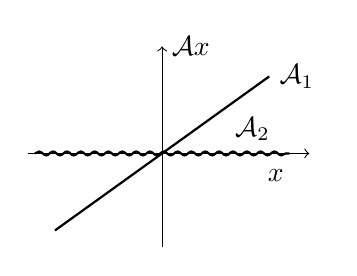
\begin{tikzpicture}[scale=0.85]
\draw[->] (-2,0) -- (2.2,0) node[right] {$\V$};
\node[below] at (1.7,-0.1) {$x$};
\draw[->] (0,-1.4) -- (0,1.6) node[right] {$\mathcal{A}x$};
\node[left] at (-0.1,1.5) {$\W$};
\draw[thick] (-1.6,-1.15) -- (1.6,1.15) node[right] {$\mathcal{A}_1$};
\draw[thick,decorate,decoration={snake,amplitude=0.7pt,segment length=5pt}] (-1.9,0) -- (1.9,0);
\node[above] at (1.35,0.05) {$\mathcal{A}_2$};
\end{tikzpicture}
\end{minipage}%
\begin{minipage}{0.4\textwidth}
\begin{align*}
\Null(\mathcal{A}_1)&=\{0_V\}\\
\Null(\mathcal{A}_2)&=\V=\R
\end{align*}
\end{minipage}
\end{center}
% corrected: notes had N(A_1) = 0_V (null space is a set: {0_V})
\explain{$\mathcal{A}_1$: a line through the origin with nonzero slope (only $x=0$ maps to $0$); $\mathcal{A}_2$: the zero map (every $x$ maps to $0$).}

\begin{claim}
\key{$\Null(\mathcal{A})$ is a subspace of $\V$.}
\end{claim}

\begin{center}
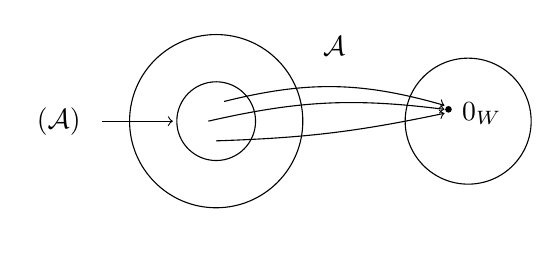
\begin{tikzpicture}
\draw (0,0) circle (1.1); \node at (0,-1.4) {$\V$};
\draw (0,0) circle (0.5);
\node at (-2.0,0) {$\Null(\mathcal{A})$};
\draw[->] (-1.45,0) -- (-0.55,0);
\draw (3.2,0) circle (0.8); \node at (3.2,-1.2) {$\W$};
\fill (2.95,0.15) circle (1.2pt); \node[right] at (3.0,0.1) {$0_W$};
\draw[->] (0.1,0.25) to[bend left=15] (2.9,0.2);
\draw[->] (-0.1,0) to[bend left=10] (2.9,0.15);
\draw[->] (0,-0.25) to[bend right=5] (2.9,0.1);
\node at (1.5,0.95) {$\mathcal{A}$};
\end{tikzpicture}
\end{center}

Let $x_1 \,\&\, x_2\in\Null(\mathcal{A})$. Show
\[
\left.\begin{aligned}
x_1+x_2 &\overset{?}{\in}\Null(\mathcal{A})\\
\alpha x_1 &\overset{?}{\in}\Null(\mathcal{A})
\end{aligned}\right\}
\Rightarrow \Null(\mathcal{A}) \text{ is a subspace.}
\]
We have $\mathcal{A}x_1=0_W$, $\mathcal{A}x_2=0_W$. Then
\begin{align*}
\mathcal{A}(x_1+x_2) &= \underbrace{\mathcal{A}x_1}_{0_W}+\underbrace{\mathcal{A}x_2}_{0_W}=0_W &&\Rightarrow\ x_1+x_2\in\Null(\mathcal{A})\\
\mathcal{A}(\alpha x_1) &= \alpha\mathcal{A}x_1=\alpha 0_W=0_W &&\Rightarrow\ \alpha x_1\in\Null(\mathcal{A})
\end{align*}
$\therefore$ $\Null(\mathcal{A})$ is closed under addition and scalar multiplication, hence a subspace of $\V$.

\begin{example}
$\V=\{\text{polynomials with degree}\le 2 \text{ on } [0,1]\}$, \quad $\W=\R$,
\[
\mathcal{A}f=\int_0^1 f(t)\,dt. \qquad\text{Find a basis for } \Null(\mathcal{A}).
\]
Let $v=at^2+bt+c$. Then
\begin{align*}
\mathcal{A}v=0_W \ &\Rightarrow\ \int_0^1(at^2+bt+c)\,dt=0\\
&\Rightarrow\ \left.\frac{at^3}{3}+\frac{bt^2}{2}+ct\right|_0^1=\frac a3+\frac b2+c=0\\
&\Rightarrow\ c=-\frac a3-\frac b2, \qquad \dim\Null(\mathcal{A})=2
\end{align*}
% ===== Page 27 =====
Hence\origpage{27}
\begin{align*}
at^2+bt+c &= at^2+bt-\frac a3-\frac b2\\
&= a\left(t^2-\frac13\right)+b\left(t-\frac12\right)
\end{align*}
A basis for $\Null(\mathcal{A})$: $\left\{t^2-\frac13,\ t-\frac12\right\}$.
\explain{Check: $\int_0^1(t^2-\frac13)\,dt=\frac13-\frac13=0$, $\int_0^1(t-\frac12)\,dt=\frac12-\frac12=0$; the two polynomials have different degrees, so they are linearly independent. Consistent with rank--nullity: $\dim\V=3=\dim\Null(\mathcal{A})+\dim\Range(\mathcal{A})=2+1$.}
\end{example}

\subsection{One-to-One Transformations}\label{ss:one-to-one}

\begin{definition}
A linear transformation $\mathcal{A}:\V\to\W$ is called \term{one-to-one} iff
\[
\mathcal{A}v_1=\mathcal{A}v_2 \quad\text{implies}\quad v_1=v_2.
\]
\end{definition}

\begin{center}
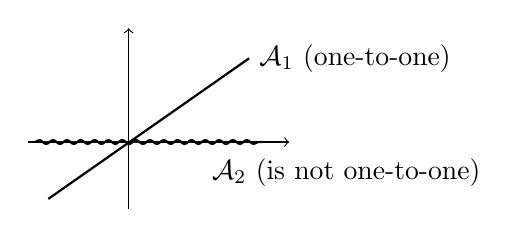
\begin{tikzpicture}[scale=0.85]
\draw[->] (-1.5,0) -- (2.4,0);
\draw[->] (0,-1) -- (0,1.7);
\draw[thick] (-1.2,-0.85) -- (1.8,1.25) node[right] {$\mathcal{A}_1$ (one-to-one)};
\draw[thick,decorate,decoration={snake,amplitude=0.7pt,segment length=5pt}] (-1.4,0) -- (2.0,0);
\node[right] at (1.1,-0.45) {$\mathcal{A}_2$ (is not one-to-one)};
\end{tikzpicture}
\end{center}

\begin{proposition}
A linear transformation $\mathcal{A}:\V\to\W$ is \key{one-to-one iff $\Null(\mathcal{A})=\{0_V\}$}:
\[
\text{one-to-one} \ \iff\ \Null(\mathcal{A})=\{0_V\}
\ \iff\ \dim\Null(\mathcal{A})=\underline{\underline{0}}.
\]
\end{proposition}
% note: in the notes, the second equivalence is written as stacked "<= , =>" arrows under the first one.

\needspace{6\baselineskip}
\paragraph{Proof techniques.}
\begin{align*}
&p\Rightarrow q && \text{(constructive proof)}\\
&\bar q\Rightarrow \bar p && \text{(contraposition proof)}\\
&p\wedge \bar q=\text{False} && \text{(contradiction proof)}
\end{align*}

\begin{proof}
\textbf{One-to-one $\Rightarrow \Null(\mathcal{A})=\{0_V\}$.}
We use contraposition ($p\Rightarrow q$ \ $\equiv$ \ $\bar q\Rightarrow \bar p$), i.e.\ we show
\[
\Null(\mathcal{A})\ne\{0_V\} \ \Rightarrow\ \text{not one-to-one.}
\]
\begin{align*}
&\exists x\ne 0_V \text{ s.t. } x\in\Null(\mathcal{A}), \quad\text{i.e. } \mathcal{A}x=0_W.\\
&\text{Let } v_1\in\V \text{ and } v_2=v_1+x\in\V. \quad\text{As } x\ne 0_V \Rightarrow v_2\ne v_1.\\
&\mathcal{A}v_2=\mathcal{A}v_1+\underbrace{\mathcal{A}x}_{0_W}=\mathcal{A}v_1
  \ \Rightarrow\ \mathcal{A} \text{ is not one-to-one.}
\end{align*}

\textbf{$\Null(\mathcal{A})=\{0_V\}\Rightarrow$ one-to-one.}
Again by contraposition: not one-to-one $\Rightarrow \Null(\mathcal{A})\ne\{0_V\}$.
\begin{align*}
&\exists v_1\ne v_2 \text{ s.t. } \mathcal{A}v_1=\mathcal{A}v_2\\
&\Rightarrow\ \mathcal{A}v_1-\mathcal{A}v_2=0_W\\
&\Rightarrow\ \mathcal{A}(v_1-v_2)=0_W\\
&\Rightarrow\ 0_V\ne v_1-v_2\in\Null(\mathcal{A})\\
&\Rightarrow\ \Null(\mathcal{A})\ne\{0_V\} \qedhere
\end{align*}
\end{proof}
\begin{insight}[Why the null space decides injectivity]
For a linear map, $\mathcal{A}v_1=\mathcal{A}v_2\iff\mathcal{A}(v_1-v_2)=0_W\iff v_1-v_2\in\Null(\mathcal{A})$. So the set of vectors with the same image as $v_1$ is the shifted copy $v_1+\Null(\mathcal{A})$; images are unique exactly when this copy is the single point $v_1$, i.e.\ when $\Null(\mathcal{A})=\{0_V\}$.
\end{insight}

% ===== Page 28 =====
\begin{example}\origpage{28}
$\V=\W=\{\text{polynomials with degree}\le 2\}$, \quad $\mathcal{A}=\dfrac{d}{dt}$. \quad Is $\mathcal{A}$ one-to-one?
\begin{align*}
&\mathcal{A}(at^2+bt+c)=2at+b=0_W=0(t) \ \Rightarrow\ a=0,\ b=0\\
&\Null(\mathcal{A})=\{c\}=\{\text{constant polynomials}\}, \qquad \dim\Null(\mathcal{A})=1\\
&\Null(\mathcal{A})\ne\{0_V\}\ \Rightarrow\ \text{\key{Not one-to-one}}
\end{align*}
\explain{Side note in the notes: $\Range(\mathcal{A})=\{\text{poly.\ degree}\le 1\}=\Span\{1,t\}$ (2 elements, $\dim\Range(\mathcal{A})=2$).}
% corrected: notes had the side note labelled N(A) = {poly degree <= 1}; this is the range of d/dt (cf. p.29), the null space is the constants
\end{example}

\begin{example}\label{ex:integral-not-1-1}
$\V=\{f\mid f:[0,1]\to\R,\ f \text{ is integrable}\}$, \quad $\W=\R$,
\[
\mathcal{A}f=\int_0^1 f(t)\,dt. \qquad\text{Is } \mathcal{A} \text{ one-to-one?}
\]
Take
\[
f(t)=2t-1\ne 0_V, \qquad \mathcal{A}f=\left(t^2-t\right)\Big|_0^1=0.
\]
$\therefore$ Not one-to-one. \quad ($\dim\Null(\mathcal{A})=\infty$)
\explain{E.g.\ $t^k-\frac{1}{k+1}$, $k=1,2,3,\dots$ all integrate to $0$ and are linearly independent, so the null space is infinite dimensional.}
\end{example}

\needspace{9\baselineskip}
\begin{example}
$\V=\W=\R^2$, \quad $x=\bmat{\alpha_1\\ \alpha_2}$, \quad $\mathcal{A}x=\bmat{\alpha_1\\ \alpha_1+\alpha_2}$. \quad Is $\mathcal{A}$ one-to-one?
\begin{align*}
&\mathcal{A}x=\bmat{0\\0}=\bmat{\alpha_1\\ \alpha_1+\alpha_2} \ \Rightarrow\ \alpha_1=\alpha_2=0\\
&\Null(\mathcal{A})=\left\{\bmat{0\\0}\right\} \ \checkmark \qquad
\cancel{\Null(\mathcal{A})=\bmat{0\\0}}
\end{align*}
\explain{Crossed out: $\Null(\mathcal{A})$ is a subspace (a set), whereas $\left[\begin{smallmatrix}0\\0\end{smallmatrix}\right]$ alone is not a set/subset --- write it inside braces.}
\end{example}

\subsection{Range Space, Onto Transformations and the Rank--Nullity Theorem}\label{ss:range}

\begin{definition}
Let $\mathcal{A}:\V\to\W$ be a linear transformation. The \term{range space} of $\mathcal{A}$ is defined as
\[
\Range(\mathcal{A})\triangleq\{w\in\W\mid \exists v\in\V \text{ s.t. } \mathcal{A}v=w\}.
\]
\end{definition}

\begin{claim}
\key{$\Range(\mathcal{A})$ is a subspace of $\W$.}
\end{claim}
Let $w_1,w_2\in\Range(\mathcal{A})$. By the definition of range space,
\begin{align*}
&\exists v_1,v_2 \text{ s.t. } \mathcal{A}v_1=w_1, \quad \mathcal{A}v_2=w_2\\
&\mathcal{A}(v_1+v_2)=\mathcal{A}v_1+\mathcal{A}v_2=w_1+w_2 \ \Rightarrow\ w_1+w_2\in\Range(\mathcal{A})\\
&\mathcal{A}(\alpha v_1)=\alpha\mathcal{A}v_1=\alpha w_1 \ \Rightarrow\ \alpha w_1\in\Range(\mathcal{A})
\end{align*}
% corrected: notes had "alpha w_1 = A(alpha v_1) = alpha A v_1 = alpha w_1 in R(A)" (circular chain); rewritten as an implication
$\therefore$ $\Range(\mathcal{A})$ is closed under addition and scalar multiplication, hence a subspace of $\W$.

% ===== Page 29 =====
\begin{example}\origpage{29}
$\V=\W=\R$.
\begin{center}
\begin{minipage}{0.36\textwidth}\centering
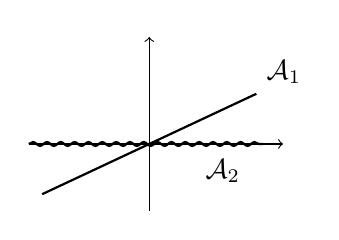
\begin{tikzpicture}[scale=0.85]
\draw[->] (-1.8,0) -- (2,0) node[right] {$\V$};
\draw[->] (0,-1) -- (0,1.6) node[left] {$\W$};
\draw[thick] (-1.6,-0.75) -- (1.6,0.75) node[above right] {$\mathcal{A}_1$};
\draw[thick,decorate,decoration={snake,amplitude=0.7pt,segment length=5pt}] (-1.8,0) -- (1.7,0);
\node at (1.1,-0.4) {$\mathcal{A}_2$};
\end{tikzpicture}
\end{minipage}%
\begin{minipage}{0.6\textwidth}
\begin{align*}
\Null(\mathcal{A}_1)&=\{0\}, & \dim\Null(\mathcal{A}_1)&=0\\
\Null(\mathcal{A}_2)&=\V=\R, & \dim\Null(\mathcal{A}_2)&=1\\
\Range(\mathcal{A}_1)&=\W=\R, & \dim\Range(\mathcal{A}_1)&=1\\
\Range(\mathcal{A}_2)&=\{0\}, & \dim\Range(\mathcal{A}_2)&=0
\end{align*}
\end{minipage}
\end{center}
% corrected: notes had "dim R(A_1) = 0" in the last line; A_2 is meant.
\explain{$\dim\Null(\mathcal{A}_1)+\dim\Range(\mathcal{A}_1)=0+1=1$, \quad $\dim\Null(\mathcal{A}_2)+\dim\Range(\mathcal{A}_2)=1+0=1$.}
\end{example}

\begin{definition}
A linear transformation $\mathcal{A}:\V\to\W$ is called \term{onto} iff \key{$\Range(\mathcal{A})=\W$}; otherwise, if $\Range(\mathcal{A})\ne\W$ (i.e.\ $\Range(\mathcal{A})\subsetneq\W$), $\mathcal{A}$ is called \term{into}.
% corrected: notes had "R(A) \not\subseteq W"; R(A) is always a subset of W, so "proper subset" (\subsetneq) is meant
\end{definition}

\begin{example}
$\V=\W=\{\text{polynomials with degree}\le 2\}$ \ ($\to\dim 3$),
\[
\mathcal{A}=\frac{d}{dt}, \qquad \mathcal{A}(at^2+bt+c)=2at+b.
\]
\begin{align*}
\Null(\mathcal{A})&=\{\text{constant polynomials}\}, & \dim\Null(\mathcal{A})&=1\\
\Range(\mathcal{A})&=\{\text{polynomials with degree}\le 1\}, & \dim\Range(\mathcal{A})&=2
\end{align*}
$\Range(\mathcal{A})\ne \W \ \Rightarrow\ \therefore \mathcal{A}$ is not onto.
\explain{Sum: $1+2=3$, the same as $\dim \V$.}
\end{example}

\begin{example}
$\V=\{f\mid f:[0,1]\to\R,\ f \text{ is integrable}\}$, \quad $\W=\R$,
\[
\mathcal{A}f=\int_0^1 f(t)\,dt, \qquad \Range(\mathcal{A})=\R.
\]
\explain{For any $c\in\R$, the constant function $f(t)=c$ gives $\mathcal{A}f=c$, so $\mathcal{A}$ is onto (but not one-to-one, see Example~\ref{ex:integral-not-1-1}).}
\end{example}

\sep
\[
\left.\begin{aligned}
\dim\Null(\mathcal{A}) &\triangleq \text{\term{nullity}}\\
\dim\Range(\mathcal{A}) &\triangleq \text{\term{rank}}
\end{aligned}\right\}\overset{+}{\longrightarrow} \text{constant}
\]

\begin{theorem}[Rank--Nullity Theorem]
If $\V$ is finite dimensional and $\mathcal{A}$ is a linear transformation from $\V$ into $\W$, then $\Range(\mathcal{A})$ is finite dimensional and \key{nullity $+$ rank $=\dim\V$}:
\[
\dim\Null(\mathcal{A})+\dim\Range(\mathcal{A})=\dim\V .
\]
\end{theorem}
\begin{insight}[Proof sketch and consequences]
Take a basis $\{u_1,\dots,u_r\}$ of $\Null(\mathcal{A})$ and extend it to a basis $\{u_1,\dots,u_r,v_{r+1},\dots,v_n\}$ of $\V$. Then $\Range(\mathcal{A})=\Span\{\mathcal{A}v_{r+1},\dots,\mathcal{A}v_n\}$ (since $\mathcal{A}u_i=0_W$), and these $n-r$ images are linearly independent: $\sum\beta_j\mathcal{A}v_j=0_W\Rightarrow\sum\beta_jv_j\in\Null(\mathcal{A})\Rightarrow$ all $\beta_j=0$. Hence $\dim\Range(\mathcal{A})=n-r$.

Consequences: $\mathcal{A}$ one-to-one $\iff$ $\dim\Range(\mathcal{A})=\dim\V$; and if $\dim\V=\dim\W<\infty$, then one-to-one $\iff$ onto. In the examples above: $\frac{d}{dt}$ on polynomials of degree $\le2$: nullity $+$ rank $=1+2=3=\dim\V$, so it is neither one-to-one nor onto.
\end{insight}

\subsection{Matrix Representations}\label{ss:matrix-rep}

\begin{definition}
Let $\V$ ($\dim=n$) and $\W$ ($\dim=m$) be two linear spaces over the same field $\F$.
Let $\mathcal{A}:\V\to\W$ be a linear transformation. Given the bases $B=\{v_1,v_2,\dots,v_n\}$ and $C=\{w_1,w_2,\dots,w_m\}$ for $\V$ and $\W$, the transformation can be represented by a matrix $A=[a_{ij}]$ ($a_{ij}\in\F$), its \term{matrix representation}, s.t.
\[
[w]_C=A\,[v]_B
\]
for any $w,v$ satisfying $w=\mathcal{A}v$.
\end{definition}
\explain{$A$ is $m\times n$; its $j$th column is the coordinate vector $[\mathcal{A}v_j]_C$ (procedure below). The matrix depends on the chosen bases $B$ and $C$.}

% ===== Page 30 =====
\needspace{16\baselineskip}
\begin{example}\origpage{30}
\begin{align*}
\V&=\{\text{polynomials with degree}\le 3\}, \qquad
\W=\{\text{polynomials with degree}\le 2\}\\
\mathcal{A}&:\V\to\W, \qquad \mathcal{A}f=\frac{df}{dt}\\
B&=\{\underbrace{1}_{v_1},\ \underbrace{1+t}_{v_2},\ \underbrace{1+t+t^2}_{v_3},\ \underbrace{1+t+t^2+t^3}_{v_4}\}\\
C&=\{\underbrace{1}_{w_1},\ \underbrace{1+t}_{w_2},\ \underbrace{1+t+t^2}_{w_3}\}\\
[w]_C&=A\,[v]_B \qquad\text{e.g. } [v]_B=\bmat{1\\0\\0\\0}
\end{align*}

\paragraph{Procedure.}
\begin{itemize}[label=$*$]
\item Choose $v=v_j$ for $j=1,\dots,n$:
\[
[v]_B=e_j=\bmat{0\\0\\ \vdots\\ 1\\ \vdots\\ 0}\leftarrow j\text{th element}
\]
\explain{$A\,e_j$ picks out the $j$th column of $A$: this gives the first column for $j=1$, and in general the $j$th column.}
\item Find $w=\mathcal{A}v_j$.
\item \key{$j$th column of $A$ is $[\mathcal{A}v_j]_C$.}
\end{itemize}

\paragraph{Columns of $A$.}
\begin{align*}
v=v_1:\quad [v_1]_B&=\bmat{1\\0\\0\\0}, & \mathcal{A}v_1&=0=0w_1+0w_2+0w_3 &&\Rightarrow\ 1^{\text{st}} \text{ column of } A \text{ is } \bmat{0\\0\\0}\\[4pt]
v=v_2:\quad [v_2]_B&=\bmat{0\\1\\0\\0}, & \mathcal{A}v_2&=1=1w_1+0w_2+0w_3 &&\Rightarrow\ 2^{\text{nd}} \text{ column of } A \text{ is } \bmat{1\\0\\0}\\[4pt]
v=v_3:\quad [v_3]_B&=\bmat{0\\0\\1\\0}, & \mathcal{A}v_3&=2t+1=-w_1+2w_2+0w_3 &&\Rightarrow\ 3^{\text{rd}} \text{ column of } A \text{ is } \bmat{-1\\2\\0}\\[4pt]
v=v_4:\quad [v_4]_B&=\bmat{0\\0\\0\\1}, & \mathcal{A}v_4&=3t^2+2t+1 &&\\*
&& &=-1w_1-1w_2+3w_3 &&\Rightarrow\ 4^{\text{th}} \text{ column of } A \text{ is } \bmat{-1\\-1\\3}
\end{align*}
\[
\boxed{A=\bmat{0&1&-1&-1\\0&0&2&-1\\0&0&0&3}}
\]
\explain{Coordinates in $C$: $2t+1=-1\cdot1+2(1+t)$; $3t^2+2t+1=3(1+t+t^2)-1\cdot(1+t)-1\cdot1$ (match the $t^2$, then $t$, then constant coefficients).}

\sep
% ===== Page 31 =====
\origpage{31}%
\paragraph{Check.} Let $v=t^3+2t^2+3t+4$. Then
\[
[v]_B=\bmat{1\\1\\1\\1}, \qquad [w]_C=A\,[v]_B=\bmat{-1\\1\\3}
\]
\begin{align*}
w&=-w_1+w_2+3w_3\\
&=-1+1+t+3+3t+3t^2=3t^2+4t+3 \quad /\!/
\end{align*}
\explain{Indeed $\frac{d}{dt}(t^3+2t^2+3t+4)=3t^2+4t+3$. ($[v]_B$: $v=1\cdot v_1+1\cdot v_2+1\cdot v_3+1\cdot v_4$, since $v_1+v_2+v_3+v_4=4+3t+2t^2+t^3$.)}
\end{example}

\subsection{Change of Basis and Similar Matrices}\label{ss:basis-change-rep}

\needspace{10\baselineskip}
\paragraph{1) Basis change in the domain.} Let $[v]_B=P\,[v]_{\bar B}$.
\begin{align*}
[w]_C&=A\,[v]_B\\
[w]_C&=\bar A\,[v]_{\bar B}\\
[w]_C&=A\cdot P\,[v]_{\bar B}
\end{align*}
\[
\therefore\ \boxed{\bar A=A\cdot P}
\]

\needspace{10\baselineskip}
\paragraph{2) Basis change in the co-domain.} Let $[w]_C=Q\,[w]_{\bar C}$.
\begin{align*}
[w]_C&=A\,[v]_B\\
[w]_{\bar C}&=\bar A\,[v]_B\\
Q\,[w]_{\bar C}&=A\,[v]_B\\
[w]_{\bar C}&=Q^{-1}A\,[v]_B
\end{align*}
\[
\therefore\ \boxed{\bar A=Q^{-1}\cdot A}
\]

\needspace{10\baselineskip}
\paragraph{3) Basis change in both domain and co-domain.} With $[v]_B=P\,[v]_{\bar B}$ and $[w]_C=Q\,[w]_{\bar C}$:
\begin{align*}
[w]_C&=A\,[v]_B\\
[w]_{\bar C}&=\bar A\,[v]_{\bar B}\\
Q\,[w]_{\bar C}&=A\,P\,[v]_{\bar B}\\
[w]_{\bar C}&=Q^{-1}AP\,[v]_{\bar B}
\end{align*}
% corrected: notes had [v]_B (no bar) in the second line; [v]_{\bar B} is meant. The last two lines are added (combine 1) and 2)).
\[
\therefore\ \boxed{\bar A=Q^{-1}AP}
\]

\needspace{9\baselineskip}
\paragraph{Special case.}
If $\V=\W$, $\mathcal{A}$ is a linear transformation from $\V$ into $\V$. Then the basis $B$ can be taken to be the same as $C$. Then a basis change in both the domain and co-domain would give
\[
\therefore\ \boxed{\bar A=P^{-1}AP}
\]
\explain{Here $Q=P$ since the same basis change is applied to domain and co-domain; $A$ and $\bar A$ are then called \term{similar} matrices.}

\begin{example}
\begin{align*}
\V&=\{\text{polynomials with degree}\le 3\}, & B&=\{1,\ 1+t,\ 1+t+t^2,\ 1+t+t^2+t^3\}\\
\W&=\{\text{polynomials with degree}\le 2\}, & C&=\{1,\ 1+t,\ 1+t+t^2\}
\end{align*}
\[
A=\bmat{0&1&-1&-1\\0&0&2&-1\\0&0&0&3}
\]

% ===== Page 32 =====
\begin{itemize}[label=$*$]
\item\origpage{32}Change the basis in the domain to $\bar B=\{1,t,t^2,t^3\}$:
\[
\bar A=AP, \qquad [v]_B=P\,[v]_{\bar B}
\]
\[
P=\bmat{1&-1&0&0\\0&1&-1&0\\0&0&1&-1\\0&0&0&1},
\qquad
\bar A=AP=\bmat{0&1&-2&0\\0&0&2&-3\\0&0&0&3}
\]
\explain{Column $j$ of $P$ is $[\bar v_j]_B$: $1=v_1$, $t=v_2-v_1$, $t^2=v_3-v_2$, $t^3=v_4-v_3$. Check of $\bar A$: $\frac{d}{dt}t^2=2t=-2\cdot1+2(1+t)$ and $\frac{d}{dt}t^3=3t^2=3(1+t+t^2)-3(1+t)$, matching columns 3 and 4.}
\item Change the basis in the co-domain to the canonical basis $\bar C=\{1,t,t^2\}$, while keeping the canonical basis $\bar B$ in the domain:
\begin{align*}
[w]_{\bar C}&=\bar{\bar A}\,[v]_{\bar B}\\
\bar{\bar A}&=Q^{-1}\bar A, && [w]_C=Q\,[w]_{\bar C}\\
\bar{\bar A}&=Q^{-1}\bar A, && R\,[w]_C=[w]_{\bar C}\\
\bar{\bar A}&=R\bar A, && [w]_{\bar C}=R\,[w]_C
\end{align*}
% corrected: notes had the first "\bar{\bar A} = Q^{-1}\bar A" line with a single bar on the left (double bar meant).
\[
R=\bmat{1&1&1\\0&1&1\\0&0&1}=Q^{-1},
\qquad
\bar{\bar A}=\bmat{0&1&0&0\\0&0&2&0\\0&0&0&3}
\]
\explain{$Q^{-1}\bar A$ $\Rightarrow$ linear combinations of rows of $\bar A$ (row 1 $=$ rows $1+2+3$, row 2 $=$ rows $2+3$, row 3 unchanged). Column $j$ of $R$ is $[w_j]_{\bar C}$: $1$, $1+t$, $1+t+t^2$.}
\begin{insight}[Check]
$\bar{\bar A}$ is the matrix of $\frac{d}{dt}$ in the canonical bases: $1\mapsto0$, $t\mapsto1$, $t^2\mapsto2t$, $t^3\mapsto3t^2$, which gives exactly the columns $\bmat{0\\0\\0},\bmat{1\\0\\0},\bmat{0\\2\\0},\bmat{0\\0\\3}$. Altogether $\bar{\bar A}=Q^{-1}AP=RAP$.
\end{insight}
\end{itemize}
\end{example}

\needspace{16\baselineskip}
\section{Direct Sums and Orthogonal Projections}\label{sec:direct-sum}
\syllabusweek{Week 6 --- direct sum decompositions, projection theorem, orthogonal projections}

\subsection{Direct Sums}\label{ss:direct-sums}

\begin{definition}
Let $\V$ be a vector space and let $M_1,\dots,M_k$ be subspaces of $\V$. The \term{sum} of these subspaces is defined as
\[
M=M_1+M_2+\dots+M_k=\{m\in\V \mid m=m_1+m_2+\dots+m_k,\ m_i\in M_i\ \forall i\}.
\]
The subspaces are called \term{linearly independent} iff
\[
m_1+m_2+\dots+m_k=0_V \quad\text{where } m_i\in M_i\ \forall i
\quad\Rightarrow\quad m_1=m_2=\dots=m_k=0_V .
\]
\end{definition}

\begin{center}
\begin{minipage}{0.42\textwidth}\centering
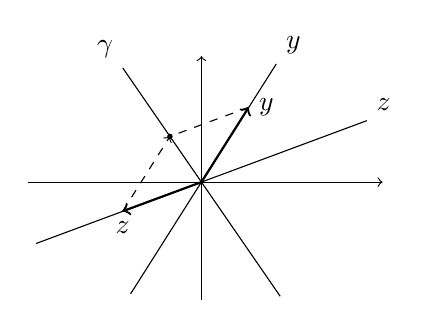
\begin{tikzpicture}[scale=1.0]
% axes
\draw[->] (-2.2,0) -- (2.3,0);
\draw[->] (0,-1.5) -- (0,1.6);
% subspaces (lines through the origin)
\draw (-0.9,-1.42) -- (0.95,1.5) node[above right] {$y$};
\draw (-2.1,-0.78) -- (2.1,0.78) node[above right] {$z$};
\draw (-1.0,1.45) -- (1.0,-1.45);
\node[above left] at (-1.0,1.45) {$\gamma$};
% vectors y, z and y+z = gamma
\draw[->,thick] (0,0) -- (0.6,0.95) node[right] {$y$};
\draw[->,thick] (0,0) -- (-1.0,-0.37) node[below] {$z$};
\draw[->,dashed] (-1.0,-0.37) -- (-0.4,0.58);
\draw[dashed] (0.6,0.95) -- (-0.4,0.58);
\fill (-0.4,0.58) circle (1pt);
\end{tikzpicture}
\end{minipage}%
\begin{minipage}{0.4\textwidth}
$y+z-\gamma=0$\\
$\Rightarrow$ not linearly independent
\end{minipage}
\end{center}

% ===== Page 33 =====
\begin{remark}\origpage{33}
Let $\V=M_1+M_2+\dots+M_k$ and let $M_1,\dots,M_k$ be linearly independent. Then for $x\in\V$,
\[
x=m_1+m_2+\dots+m_k, \qquad m_i\in M_i\ \forall i,
\]
\key{$m_1,m_2,\dots,m_k$ are unique.}
\end{remark}

\begin{proof}
Assume $m_1,\dots,m_k$ are not unique, i.e.\ $\exists i$ s.t.\ $m_i\ne\bar m_i$:
\begin{align*}
x&=m_1+\dots+m_k\\
x&=\bar m_1+\dots+\bar m_k\\
0_V&=\underbrace{(m_1-\bar m_1)}_{\in M_1}+\underbrace{(m_2-\bar m_2)}_{\in M_2}+\dots+\underbrace{(m_k-\bar m_k)}_{\in M_k}
\end{align*}
$\Rightarrow M_1,\dots,M_k$ are not linearly independent. \qedhere
\end{proof}

\begin{definition}
Let $M_1,\dots,M_k$ be subspaces of $\V$. Let
\begin{enumerate}[label=\roman*-)]
\item $M=M_1+M_2+\dots+M_k$
\item $M_1,M_2,\dots,M_k$ are linearly independent.
\end{enumerate}
Then $M$ is said to be the \term{direct sum} of $M_1,\dots,M_k$. This is shown as
\[
M=M_1\oplus M_2\oplus\dots\oplus M_k .
\]
\end{definition}

\begin{example}
$\V=\R^4$, \quad $x=(x_1,x_2,x_3,x_4)^T\in\R^4$.
\begin{alignat*}{3}
M_1&\triangleq\{x\in\R^4\mid x_4=x_3=0\}: &\quad &\bmat{x_1\\x_2\\0\\0}, &\quad \dim&=2\\
M_2&\triangleq\{x\in\R^4\mid x_1=x_2=0\}: & &\bmat{0\\0\\x_3\\x_4}, & \dim&=2\\
M_3&\triangleq\{x\in\R^4\mid x_1=0\}: & &\bmat{0\\x_2\\x_3\\x_4}, & \dim&=3
\end{alignat*}
\begin{align*}
M_1+M_2&=\R^4 && \Rightarrow \text{direct sum: } M_1\,\&\,M_2 \text{ linearly independent} \Rightarrow M_1\oplus M_2=\R^4\\
M_1+M_3&=\R^4 && \Rightarrow \text{not direct sum}\\
M_2+M_3&=M_3 && \Rightarrow \text{not direct sum } (M_2\subset M_3)
\end{align*}

\sep
For $M_1$ and $M_3$:
\[
\bmat{x_1\\x_2\\0\\0}+\bmat{0\\x_2'\\x_3'\\x_4'}=\bmat{0\\0\\0\\0},
\qquad\text{e.g.}\qquad
\underset{\in M_1}{\bmat{0\\1\\0\\0}}+\underset{\in M_3}{\bmat{0\\-1\\0\\0}}=\underset{0_V}{\bmat{0\\0\\0\\0}}
\]
As the two summands are nonzero, $M_1\,\&\,M_3$ are linearly dependent. $\therefore$ Not a direct sum.

$M_2\,\&\,M_3$ are linearly dependent (e.g.\ $m_2=(0,0,1,0)^T\in M_2$, $m_3=-m_2\in M_3$). $\therefore$ Not a direct sum.
\begin{insight}[Dimension test]
For two subspaces, $M_1+M_2$ is direct $\iff M_1\cap M_2=\{0_V\}\iff\dim(M_1+M_2)=\dim M_1+\dim M_2$. Here: $M_1\cap M_2=\{0\}$ and $2+2=4$ (direct); $M_1\cap M_3=\{(0,x_2,0,0)^T\}$, $2+3=5\ne4$ (not direct); $M_2\cap M_3=M_2$, $2+3\ne3$ (not direct).
\end{insight}
\end{example}

% ===== Page 34 =====
\subsection{Orthogonal Direct Sums and Orthogonal Complements}\label{ss:orth-complement}

\begin{definition}\origpage{34}
Let $\V$ be an inner product space. Two subspaces $M_1\,\&\,M_2$ are said to be \term{orthogonal} iff
\[
\inner{m_1}{m_2}=0 \qquad \forall m_1\in M_1,\ \forall m_2\in M_2 .
\]
We denote this $M_1\perp M_2$.
\end{definition}
% corrected: notes had "M_2 & M_2" in the first line; M_1 & M_2 meant.

\begin{definition}
Let $M$ be equal to $M_1+M_2+\dots+M_k$ and $M_i\perp M_j$ for $i\ne j$. Then $M$ is said to be an \term{orthogonal direct sum} of $M_1,\dots,M_k$. We show this as
\[
M=M_1\overset{\perp}{\oplus}M_2\overset{\perp}{\oplus}\dots\overset{\perp}{\oplus}M_k .
\]
If $M=\V$ then
\[
\V=M_1\overset{\perp}{\oplus}M_2\overset{\perp}{\oplus}\dots\overset{\perp}{\oplus}M_k
\]
is called an \term{orthogonal direct sum decomposition} of $\V$.
\end{definition}

\paragraph{\key{Orthogonality implies linear independence.}}
Let $\sum_{i=1}^{k}m_i=0_V$, \ $m_i\in M_i$. Then
\begin{align*}
\Big\langle\sum_{i=1}^{k}m_i,\,m_j\Big\rangle&=\inner{0_V}{m_j}=0\\
\sum_{i=1}^{k}\inner{m_i}{m_j}&=0
\end{align*}
Since $\inner{m_i}{m_j}=0$ when $i\ne j$:
\[
\inner{m_j}{m_j}=0 \ \Rightarrow\ m_j=0_V .
\]
\explain{The last step uses positive definiteness of the inner product. Since $j$ was arbitrary, all $m_j=0_V$: orthogonality implies linear independence.}

\begin{definition}
Let $M$ be a subspace of an inner product space $\V$. The \term{orthogonal complement} $M^\perp$ of the subspace is defined as
\[
M^\perp=\{x\in\V\mid \inner{x}{m}=0\ \forall m\in M\}.
\]
\end{definition}
The zero vector is orthogonal to every vector, so $0_V\in M^\perp$ always. Two examples:

\begin{center}
\begin{minipage}{0.34\textwidth}\centering
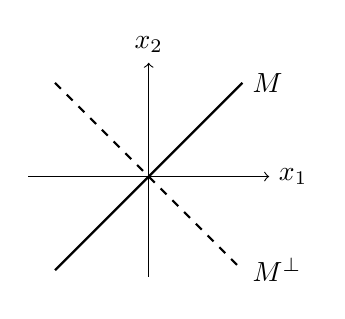
\begin{tikzpicture}[scale=0.85]
\draw[->] (-1.8,0) -- (1.8,0) node[right] {$x_1$};
\draw[->] (0,-1.5) -- (0,1.7) node[above] {$x_2$};
\draw[thick] (-1.4,-1.4) -- (1.4,1.4) node[right] {$M$};
\draw[thick,dashed] (-1.4,1.4) -- (1.4,-1.4) node[right] {$M^\perp$};
\end{tikzpicture}
\end{minipage}%
\begin{minipage}{0.6\textwidth}
\begin{align*}
M&=\Span\left\{\bmat{1\\1}\right\}, & \bmat{-1\\1}&\in M^\perp, \quad \bmat{2\\-2}\in M^\perp\\
M^\perp&=\Span\left\{\bmat{-1\\1}\right\}, & M+M^\perp&=M\overset{\perp}{\oplus}M^\perp
\end{align*}
\end{minipage}
\end{center}
\begin{center}
\begin{minipage}{0.3\textwidth}\centering
\begin{tikzpicture}[scale=0.85]
\fill[pattern=vertical lines, pattern color=gray!70] (-0.2,0) -- (2,0) -- (1.2,-1.2) -- (-1.0,-1.2) -- cycle;
\draw[->] (0,0) -- (0,2) node[above] {$z$};
\draw[->] (0,0) -- (2.3,0) node[right] {$y$};
\draw[->] (0,0) -- (-0.95,-1.45) node[below left] {$x$};
\node at (1.25,-0.75) {$M$};
\node[right] at (0,1.4) {$M^\perp$};
\end{tikzpicture}
\end{minipage}%
\begin{minipage}{0.55\textwidth}
\begin{align*}
M&=\{x\text{-}y \text{ plane}\}\\
M^\perp&=\{z \text{ axis}\}\\
\underset{\dim=2}{M}\overset{\perp}{\oplus}\underset{\dim=1}{M^\perp}&=\underset{\dim 3}{\R^3}
\end{align*}
\end{minipage}
\end{center}
Orthogonality implies linear independence, thus this is a direct sum; since the summands are also orthogonal, it is an orthogonal direct sum.

\needspace{9\baselineskip}
\begin{claim}
\key{$M^\perp$ is a subspace of $\V$.}
\end{claim}
Let $x,y\in M^\perp$, i.e.\ $\inner{x}{m}=0$, $\inner{y}{m}=0$ $\forall m\in M$. Then
\begin{align*}
\inner{x+y}{m}&=\underbrace{\inner{x}{m}+\inner{y}{m}}_{0} \quad (m\in M)\\
&=0 \quad \forall m\in M &&\Rightarrow\ x+y\in M^\perp\\
\inner{\alpha x}{m}&=\alpha\inner{x}{m}=0 \quad\forall m\in M &&\Rightarrow\ \alpha x\in M^\perp
\end{align*}
$\therefore$ $M^\perp$ is closed under addition and scalar multiplication, hence a subspace of $\V$.

% ===== Page 35 =====
\begin{theorem}[Orthogonal decomposition]\origpage{35}
Let $\V$ be an inner product space and $M$ a subspace of $\V$. Then \key{$\V$ is the orthogonal direct sum of $M$ and $M^\perp$}:
\[
\boxed{\V=M\overset{\perp}{\oplus}M^\perp}
\]
To prove this we check:
\begin{itemize}[nosep]
\item $\V=M+M^\perp$ \ (to be shown, proof below);
\item $M\,\&\,M^\perp$ are linearly independent \ $\checkmark$;
\item $M\perp M^\perp$ \ $\checkmark$.
\end{itemize}
\end{theorem}

\begin{proof}
\textbf{Part I:} $\dim M=n\triangleq\dim\V \Rightarrow M=\V$ \ \textcircled{?}\par
\explain{Answer to \textcircled{?}: a basis of $M$ consists of $n$ linearly independent vectors of $\V$; in an $n$-dimensional space any $n$ independent vectors form a basis, so they span $\V$ and $M=\V$.}

\begin{center}
\begin{minipage}{0.25\textwidth}\centering
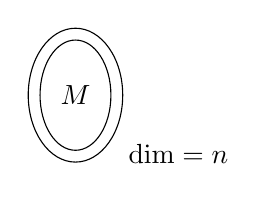
\begin{tikzpicture}
\draw (0,0) ellipse (0.6 and 0.85);
\draw (0,0) ellipse (0.45 and 0.7);
\node at (0,0) {$M$};
\node[right] at (0.55,-0.75) {$\dim\V=n$};
\end{tikzpicture}
\end{minipage}%
\begin{minipage}{0.6\textwidth}
\begin{align*}
M^\perp&=\V^\perp=\{0_V\}\\
\V&=M+M^\perp\\
x&=\underset{\in M}{x_1}+\underset{\in M^\perp}{x_2}
\ \Rightarrow\ x=\underset{\in M}{x}+\underset{\in M^\perp}{0_V} \quad\checkmark
\end{align*}
\end{minipage}
\end{center}

\textbf{Part II:} $\dim M<n$, with $\dim M = k$. Let
\begin{align*}
B&=\{m_1,m_2,m_3,\dots,m_k\} && \text{(basis for } M)\\
C&=\{m_1,m_2,\dots,m_k,m_{k+1},\dots,m_n\} && \text{(basis for } \V)
\end{align*}
Apply Gram--Schmidt orthogonalization to $C$:
\[
\bar C=\{\underbrace{\underset{\uparrow\, m_1}{e_1},e_2,\dots,e_k}_{\text{form a basis for } M},\ \overbrace{e_{k+1},\dots,e_n}^{\text{basis for } M^\perp}\},
\qquad
\Span\{e_1,\dots,e_k\}=\Span\{m_1,\dots,m_k\}.
\]
$\bar C$ is a basis for $\V$. For $x\in\V$:
\[
x=\sum_{i=1}^{n}\alpha_ie_i=\underbrace{\sum_{i=1}^{k}\alpha_ie_i}_{x_1\in M}+\underbrace{\sum_{j=k+1}^{n}\alpha_je_j}_{x_2\in M^\perp}
\]
\explain{$x_2\in M^\perp$ by construction: Gram--Schmidt makes each $e_j$ ($j>k$) orthogonal to $e_1,\dots,e_k$, which span $M$; hence $e_j\perp m$ for all $m\in M$, and so is every combination of them.}
\[
\Rightarrow\ x=\underset{\in M}{x_1}+\underset{\in M^\perp}{x_2}\ \Rightarrow\ \V=M+M^\perp \qedhere
\]
\end{proof}
\begin{insight}[The remaining two items]
The other two items are immediate: $M\perp M^\perp$ by the definition of $M^\perp$, and orthogonality implies linear independence (shown above), equivalently $M\cap M^\perp=\{0_V\}$ since $x\in M\cap M^\perp\Rightarrow\inner{x}{x}=0$. Consequently $\dim M^\perp=\dim\V-\dim M$, and $\{e_{k+1},\dots,e_n\}$ is in fact a basis of $M^\perp$. (Finite dimension of $\V$ is assumed in the proof.)
\end{insight}

\begin{example}
$\V=\R^4$,
\[
M=\Span\left\{\bmat{1\\2\\3\\4},\bmat{4\\3\\2\\1}\right\}. \qquad \text{Find a basis for } M^\perp.
\]
Complete the basis of $M$ with two canonical vectors to a basis of $\R^4$ and orthogonalize:
\[
C=\Big\{\underset{m_1}{\bmat{1\\2\\3\\4}},\ \underset{m_2}{\bmat{4\\3\\2\\1}},\ \underset{m_3}{\bmat{1\\0\\0\\0}},\ \underset{m_4}{\bmat{0\\1\\0\\0}}\Big\}
\ \xrightarrow{\text{Gram--Schmidt}}\ \bar C=\{e_1,e_2,e_3,e_4\}
\]
% corrected: notes labelled the un-orthogonalized vectors [1,0,0,0], [0,1,0,0] themselves as e_3, e_4 and wrote M^perp = sp{e_3,e_4};
% these vectors are NOT orthogonal to M (e.g. <[1,0,0,0],m_1> = 1). The last vector is cramped in the scan (could be read as 0,1,3);
% [0,1,0,0] is the reading used. The Gram--Schmidt computation below is added and verified with exact (Fraction) arithmetic.
\begin{align*}
e_1&=m_1=\bmat{1\\2\\3\\4}, \qquad \inner{e_1}{e_1}=30\\
e_2&=m_2-\frac{\inner{m_2}{e_1}}{\inner{e_1}{e_1}}e_1=\bmat{4\\3\\2\\1}-\frac{20}{30}\bmat{1\\2\\3\\4}=\frac53\bmat{2\\1\\0\\-1}\ \to\ \bmat{2\\1\\0\\-1}\\
e_3&=m_3-\frac{\inner{m_3}{e_1}}{\inner{e_1}{e_1}}e_1-\frac{\inner{m_3}{e_2}}{\inner{e_2}{e_2}}e_2
 =\bmat{1\\0\\0\\0}-\frac{1}{30}\bmat{1\\2\\3\\4}-\frac{2}{6}\bmat{2\\1\\0\\-1}=\frac1{10}\bmat{3\\-4\\-1\\2}\ \to\ \bmat{3\\-4\\-1\\2}\\
e_4&=m_4-\frac{\inner{m_4}{e_1}}{\inner{e_1}{e_1}}e_1-\frac{\inner{m_4}{e_2}}{\inner{e_2}{e_2}}e_2-\frac{\inner{m_4}{e_3}}{\inner{e_3}{e_3}}e_3\\
 &=\bmat{0\\1\\0\\0}-\frac{2}{30}\bmat{1\\2\\3\\4}-\frac{1}{6}\bmat{2\\1\\0\\-1}+\frac{4}{30}\bmat{3\\-4\\-1\\2}=\frac16\bmat{0\\1\\-2\\1}\ \to\ \bmat{0\\1\\-2\\1}
\end{align*}
\explain{Scaling a vector does not affect orthogonality, so after each step the vector is rescaled to integer entries ($\to$) and the scaled version is used in the following steps.}
\[
\boxed{M^\perp=\Span\{e_3,e_4\}=\Span\left\{\bmat{3\\-4\\-1\\2},\bmat{0\\1\\-2\\1}\right\}}
\]
\begin{insight}[Verification]
$\inner{e_3}{m_1}=3-8-3+8=0$, \ $\inner{e_3}{m_2}=12-12-2+2=0$, \ $\inner{e_4}{m_1}=2-6+4=0$, \ $\inner{e_4}{m_2}=3-4+1=0$, \ and $\inner{e_3}{e_4}=-4+2+2=0$. Since $e_3,e_4\ne0$, the set $C$ was indeed a basis of $\R^4$.

Alternatively,
\[
x\in M^\perp\iff\bmat{1&2&3&4\\4&3&2&1}x=0, \qquad\text{i.e.}\qquad M^\perp=\Null\!\left(\bmat{1&2&3&4\\4&3&2&1}\right),
\]
which has dimension $4-2=2$ and is spanned e.g.\ by $(1,-2,1,0)^T$ and $(0,1,-2,1)^T$; note $(3,-4,-1,2)^T=3(1,-2,1,0)^T+2(0,1,-2,1)^T$, so both answers describe the same subspace. Gram--Schmidt additionally gives an \emph{orthogonal} basis.
\end{insight}
\end{example}
